\documentclass[a3paper, border=20pt]{standalone}
\usepackage{tikz}
\usetikzlibrary{shapes, arrows, positioning}
\usetikzlibrary{fit}
\usetikzlibrary{matrix}
\usepackage{amsmath}

\begin{document}

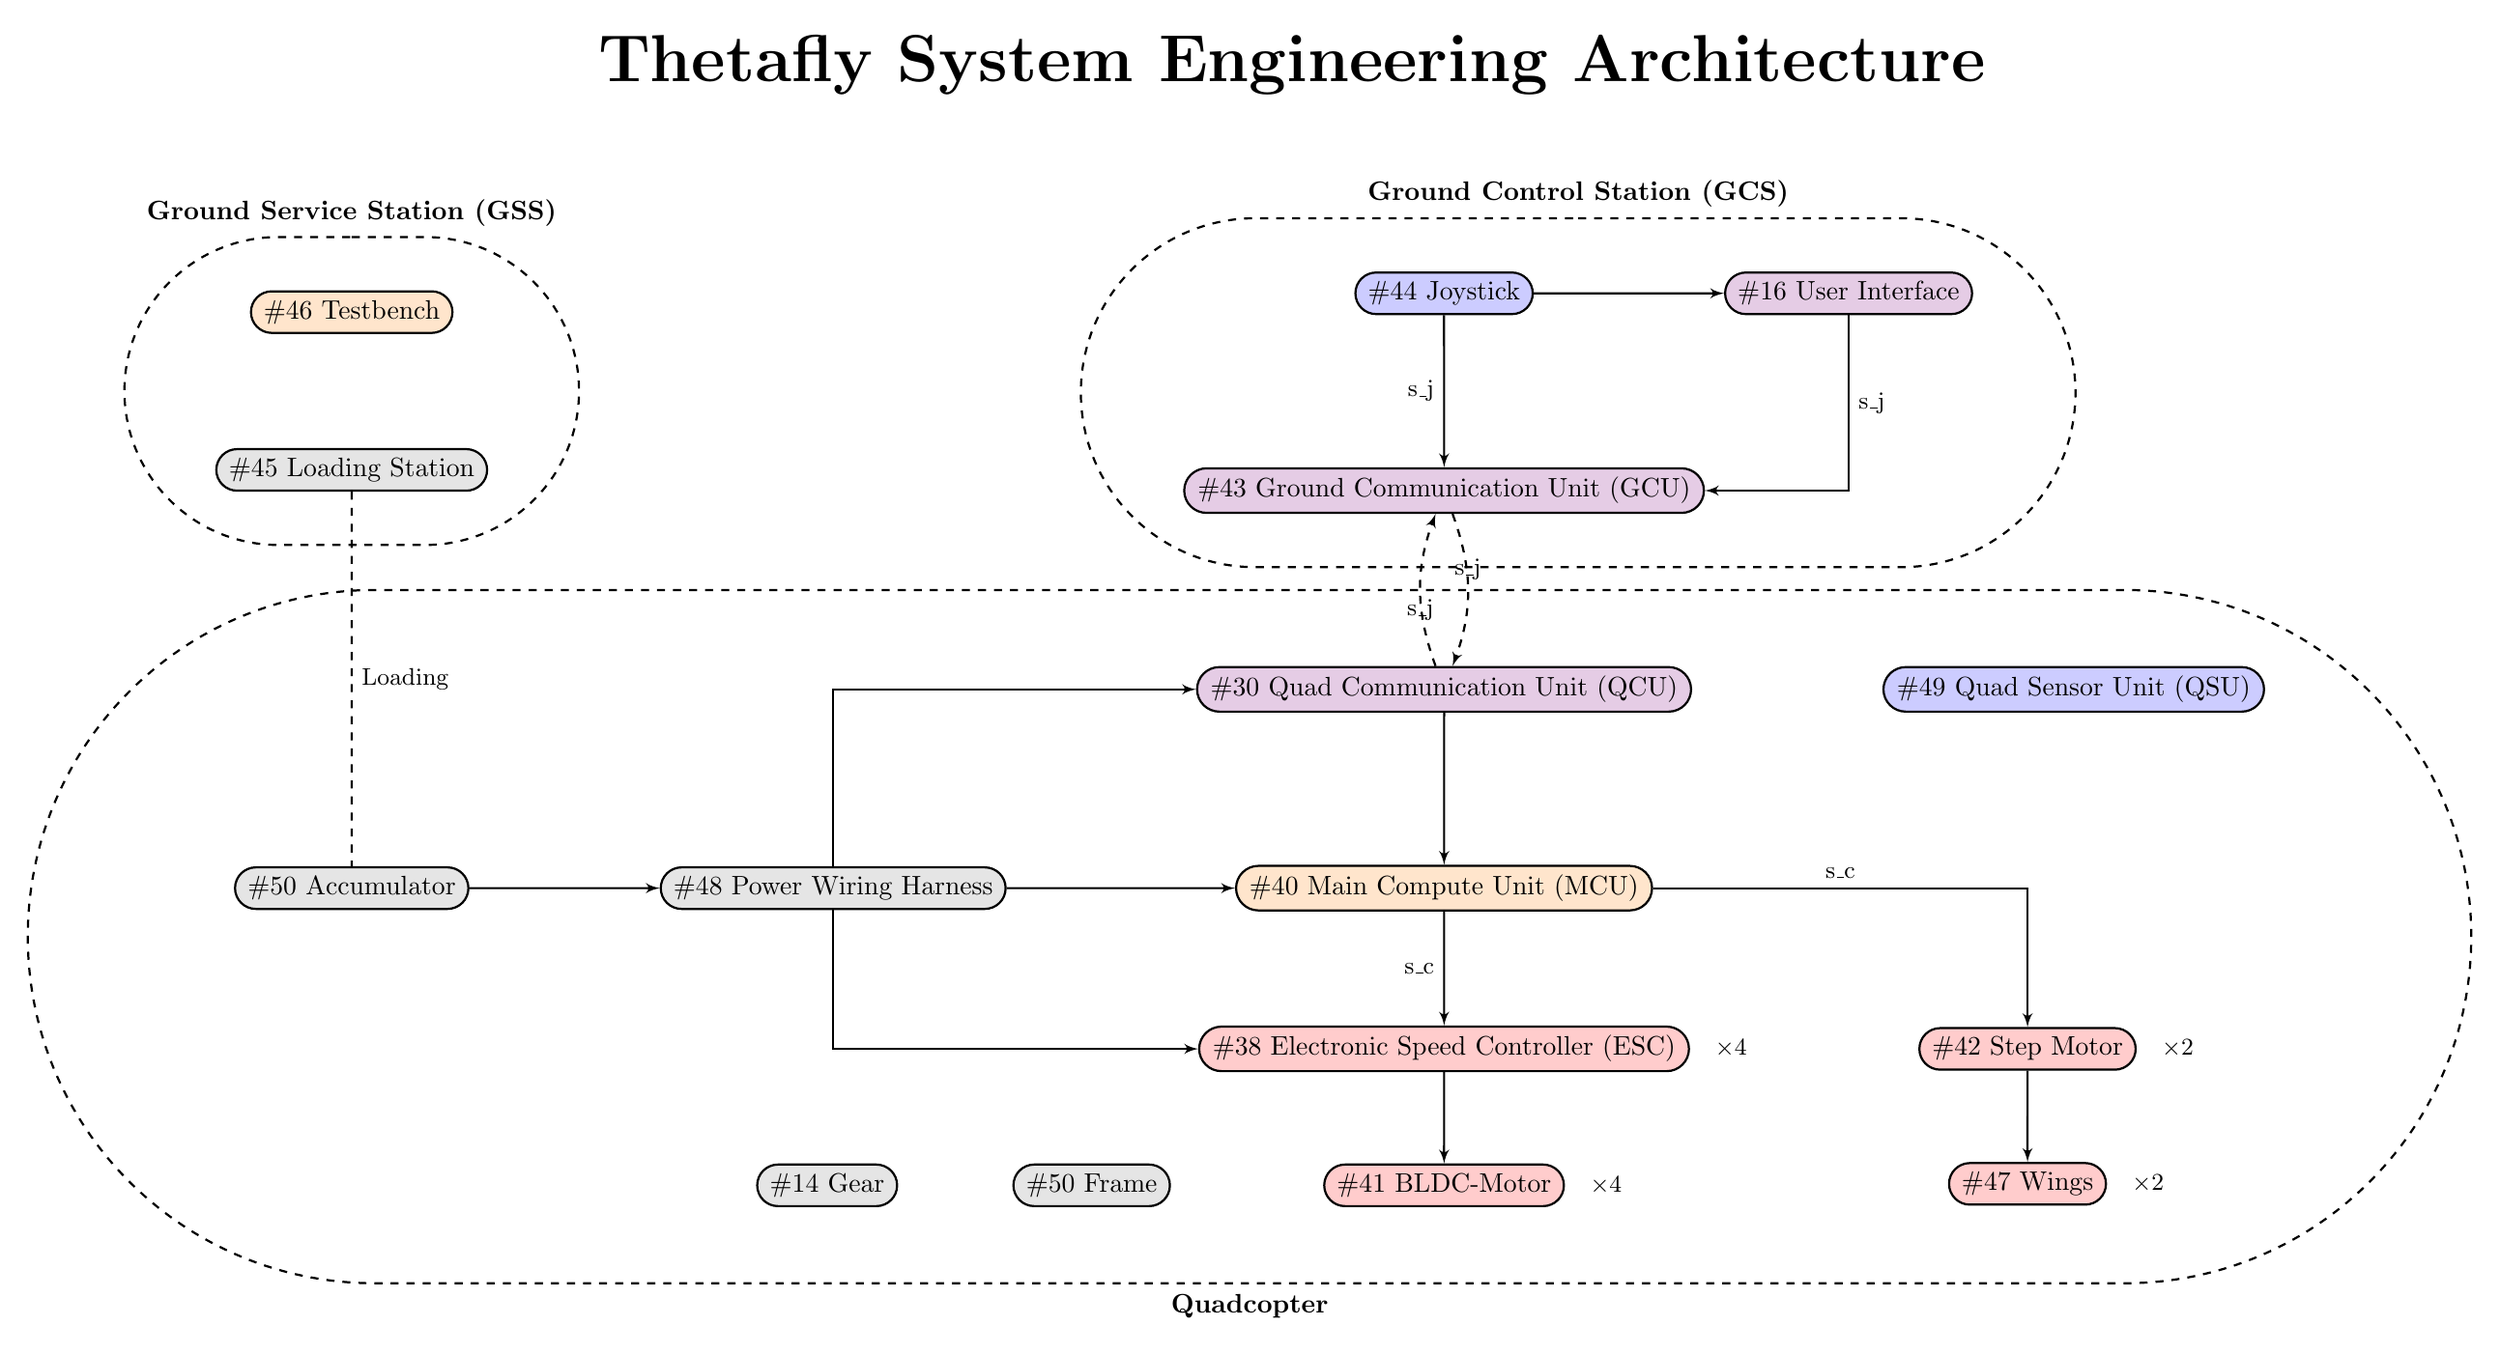
\begin{tikzpicture}[node distance=2cm, auto, >=latex', thick]
  % Titel oben zentriert
  \node[font=\Huge\bfseries] at (0,12) {Thetafly System Engineering Architecture};
  
  % Hauptdiagramm mit Offset
  \begin{scope}[xshift=2cm, yshift=9cm]
  
  % Vertikale Anordnung: Joystick, QuadUI, Communication Units, MCU
  \node[draw, rounded rectangle, fill=blue!20] (joystick) {\#44 Joystick};
  \node[draw, rounded rectangle, right=2.5cm of joystick, fill=violet!20] (quadui) {\#16 User Interface};
  \node[draw, rounded rectangle, below=2cm of joystick, fill=violet!20] (gcu) {\#43 Ground Communication Unit (GCU)};
  \node[draw, rounded rectangle, below=2cm of gcu, fill=violet!20] (rx) {\#30 Quad Communication Unit (QCU)};
  \node[draw, rounded rectangle, right=2.5cm of rx, fill=blue!20] (qsu) {\#49 Quad Sensor Unit (QSU)};
  \node[draw, rounded rectangle, below=2cm of rx, fill=orange!20, minimum width=3cm] (mcu) {\#40 Main Compute Unit (MCU)};
  
  % Power Wiring Harness
  \node[draw, rounded rectangle, fill=gray!20, left=3cm of mcu, minimum width=2.5cm] (pwh) {\#48 Power Wiring Harness};
  
  % Accumulator
  \node[draw, rounded rectangle, fill=gray!20, left=2.5cm of pwh, minimum width=2.5cm] (akku) {\#50 Accumulator};
  
  % Ground Service Station (über Accumulator, vertikal ausgerichtet)
  \node[draw, rounded rectangle, fill=orange!20, above=7cm of akku, minimum width=2.5cm] (testbench) {\#46 Testbench};
  \node[draw, rounded rectangle, fill=gray!20, below=1.5cm of testbench, minimum width=2.5cm] (ladestation) {\#45 Loading Station};
  
  \draw[dashed, thick] (ladestation) -- node[right, font=\small]{Loading} (akku);
  \draw[->, thick] (akku) -- (pwh);

  % ESC and Motor (single representation for 4 units)
  \node[draw, rounded rectangle, below=1.5cm of mcu, fill=red!20] (esc) {\#38 Electronic Speed Controller (ESC)};
  \node[draw, rounded rectangle, below=1.2cm of esc, fill=red!20] (motor) {\#41 BLDC-Motor};
  \node[right=0.2cm of esc, font=\small\bfseries] {$\times 4$};
  \node[right=0.2cm of motor, font=\small\bfseries] {$\times 4$};
  \draw[->] (mcu) -- node[left, font=\small]{s\_c} (esc);
  \draw[->] (esc) -- (motor);
  \draw[->, thick] (pwh) |- (esc);
  \draw[->, thick] (pwh) -- (mcu);
  \draw[->, thick] (pwh) |- (rx);

  % Step Motor (single representation for 2 units)
  \node[draw, rounded rectangle, right=3cm of esc, fill=red!20] (step) {\#42 Step Motor};
  \node[right=0.2cm of step, font=\small\bfseries] {$\times 2$};
  \draw[->] (mcu) -| node[near start, above, font=\small]{s\_c} (step);
  
  % Wings
  \node[draw, rounded rectangle, below=1.2cm of step, fill=red!20] (wings) {\#47 Wings};
  \node[right=0.2cm of wings, font=\small\bfseries] {$\times 2$};
  \draw[->] (step) -- (wings);

  % Frame and Gear (links von BLDC Motor, horizontal ausgerichtet, keine Verbindungen)
  \node[draw, rounded rectangle, left=2cm of motor, fill=gray!20] (frame) {\#50 Frame};
  \node[draw, rounded rectangle, left=1.5cm of frame, fill=gray!20] (gear) {\#14 Gear};

  % Connections
  \draw[->] (joystick) -- (quadui);
  \draw[->] (joystick) -- node[left, font=\small]{s\_j} (gcu);
  \draw[->] (quadui) |- node[near start, right, font=\small]{s\_j} (gcu);
  % Bidirektionale Kommunikation zwischen den Communication Units
  \draw[->, dashed, bend left=20] (gcu) to node[above, font=\small]{s\_j} (rx);
  \draw[->, dashed, bend left=20] (rx) to node[below, font=\small]{s\_j} (gcu);
  \draw[->] (rx) -- (mcu);

  % Quadcopter-Komponenten-Box
  \node[draw, dashed, rounded rectangle, fit=(mcu) (esc) (motor) (rx) (qsu) (akku) (step) (wings) (pwh) (frame) (gear), inner sep=1cm, label=below:{\textbf{Quadcopter}}] (quadbox) {};

  % Ground Control Station-Box
  \node[draw, dashed, rounded rectangle, fit=(joystick) (quadui) (gcu), inner sep=0.7cm, label=above:{\textbf{Ground Control Station (GCS)}}] (gcsbox) {};

  % Ground Service Station-Box
  \node[draw, dashed, rounded rectangle, fit=(ladestation) (testbench), inner sep=0.7cm, label=above:{\textbf{Ground Service Station (GSS)}}] (gssbox) {};
  \end{scope}
\end{tikzpicture}

% Legende
\vspace{1cm}
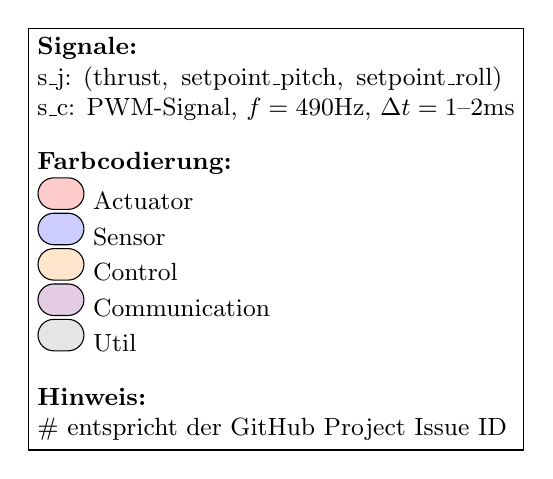
\begin{tikzpicture}
  \node[draw, rectangle, fill=white!90, font=\small, align=left] at (0,0) {
    \textbf{Signale:}\\
    s\_j: $(\text{thrust},\ \text{setpoint\_pitch},\ \text{setpoint\_roll})$\\
    s\_c: PWM-Signal, $f=490$Hz, $\Delta t=1$--$2$ms\\[0.3cm]
    \textbf{Farbcodierung:}\\
    \tikz\node[draw, rounded rectangle, fill=red!20, minimum width=0.8cm, minimum height=0.4cm] {};\ Actuator\\
    \tikz\node[draw, rounded rectangle, fill=blue!20, minimum width=0.8cm, minimum height=0.4cm] {};\ Sensor\\
    \tikz\node[draw, rounded rectangle, fill=orange!20, minimum width=0.8cm, minimum height=0.4cm] {};\ Control\\
    \tikz\node[draw, rounded rectangle, fill=violet!20, minimum width=0.8cm, minimum height=0.4cm] {};\ Communication\\
    \tikz\node[draw, rounded rectangle, fill=gray!20, minimum width=0.8cm, minimum height=0.4cm] {};\ Util\\[0.3cm]
    \textbf{Hinweis:}\\
    \# entspricht der GitHub Project Issue ID
  };
\end{tikzpicture}
\end{document}